\documentclass[a4paper, 12pt]{article}
\usepackage[utf8]{inputenc}
\usepackage[english, russian]{babel}
\usepackage{amsmath}
\usepackage{caption}
\usepackage{enumerate}
\usepackage{graphicx}
\usepackage{tikz}
\setcounter{tocdepth}{2}
\usepackage{amsfonts}
\usepackage{amssymb}

\usepackage{mathtools}
\usepackage{float}
\IfFileExists{pscyr.sty}
{
% Хак с шрифтами
\usepackage{times}
\usepackage{mathptmx}
\usepackage{pscyr}
\def\rmdefault{ftm}
\def\sfdefault{ftx}
\def\ttdefault{fer}
\DeclareMathAlphabet{\mathbf}{OT1}{ftm}{bx}{it} % bx/it or bx/m
}
% else
{
\typeout{RFDstyle message: no PScyr, shall do without...}
}
\usepackage[
  a4paper, mag=1000, includefoot,
  left=3cm, right=1.5cm, top=2cm, bottom=2cm, headsep=1cm, footskip=1cm
]{geometry}
\graphicspath {{pics/}}

\def\pa{{\partial}}
\DeclarePairedDelimiter\norm{\lVert}{\rVert}

\begin{document}
\title{Способ построения сетки для ромба с вырезом внутри в центре в виде ромба, со сторонами
выреза, параллельными сторонам ромба}
\author{Бобровников~М.~Р.}
\date{}
\maketitle
Сетка для квадрата:
\begin{figure}[H]
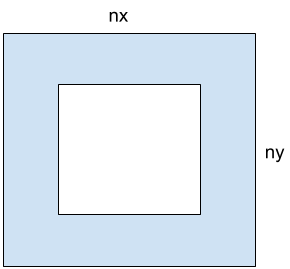
\includegraphics[]{paint}
    \end{figure}
При помощи линейного отображения сетка для квадрата растягивается на любой ромб.
Вырез задается коэффициентом подобия внутреннего ромба к внешнему.

Задание ромба:
\begin{figure}[H]
    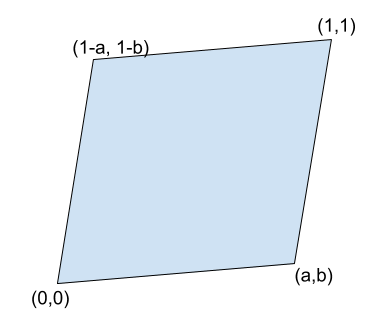
\includegraphics[]{paint2}
        \end{figure}
        Сетка разбивается следующим образом на границе с вырезом.
Вырез с коеффициентом 0.5:
\begin{figure}[H]
    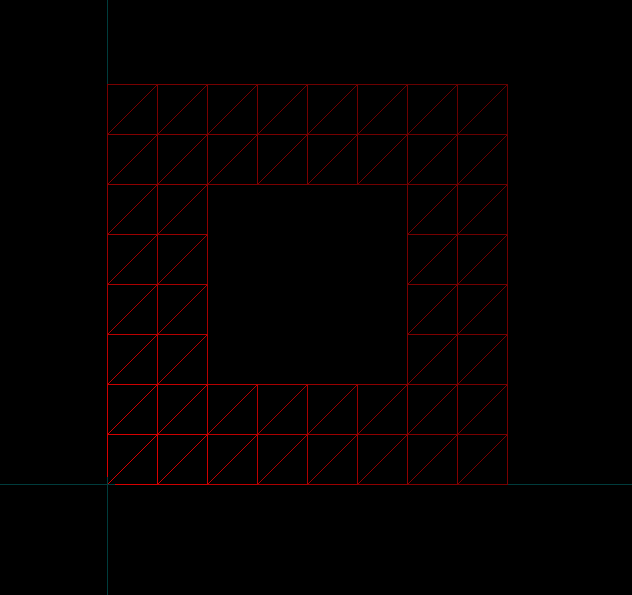
\includegraphics[width=0.7\linewidth]{coef_0_5}
        \end{figure}
Вырез с коеффициентом 0.333:
\begin{figure}[H]
    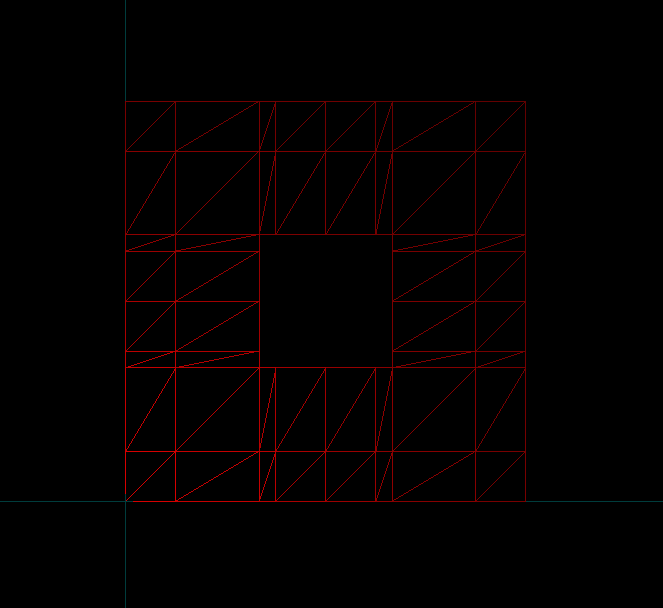
\includegraphics[width=0.7\linewidth]{coef_0_333}
        \end{figure}
\end{document}
